\section{Аналитический раздел}

В данном разделе описываются медицинские методы томографии. Рассматриваются задачи распознавания образов и нахождения объектов на изображении. Рассматривается технология нейронных сетей, приводится обзор принципа работы нейронных сетей. Описываются виды нейронных сетей, их применение в задачах классификации и сегментации. Дается обзор существующих методов распознавания и нахождения объектов на изображении.

\subsection{Томография в медицине}

Томография основана на получении послойных изображений объекта исследований. Впервые этот метод был разработан Н.И. Пироговым. Современная томография также основана на получении послойных изображений. Однако, современная томография позволяет проводить прижизненные исследования и с помощью математической обработки производить трехмерную реконструкцию изображения исследуемого органа.

В медицине используются различные методы томографии: компьютерная томография (КТ), магнитно--резонансная томография (МРТ), однофотонная эмиссионная компьютерная томография (ОЭФКТ) и позитронная эмиссионная томография (ПЭТ).

В контексте работы будут рассмотрены магнитно--резонансная и компьютерная томографии, как наиболее информативные и высокоточные методы инструментальной диагностики \cite{ctmrt}.

\subsubsection{Компьютерная томография}

Компьютерная томография (КТ) --- это способ получения послойных срезов тела человека или другого объека с помощью рентгеновских лучей. Этот метод для диагностических целей был предложен к использованию в 1972 году, его основателями принято считать Годфри Хаунсфилда и Алана Кормака, получившими за свои разработки Нобелевскую премию. В основе компьютерной томографии лежит измерение разницы ослабления рентгеновского излучения различными тканями, обработка полученных данных компьютером с помощью математических алгоритмов и формирование графического отображения (срезов) органов человека на экране с последующей их интерпретацией врачом--радиологом.

Для получения среза трубка оборачивается вокруг пациента на 360 градусов, толщина среза при этом задается заранее. В обычном КТ--сканере трубка вращается постоянно, излучение расходится веерообразно. Рентгеновская трубка и принимающее устройство (детектор) спарены, их вращение вокруг сканируемой зоны происходит синхронно: рентгеновское излучение испускается и улавливается детекторами, расположенными на противоположной стороне, практически одновременно. Веерообразное расхождение происходит под углом от 40 до 60 градусов, в зависимости от конкретного аппарата \cite{ct}.

На рисунке \ref{fig:ct} представлен принцип работы компьютерного томографа.

\begin{figure}[H]
	\centering
	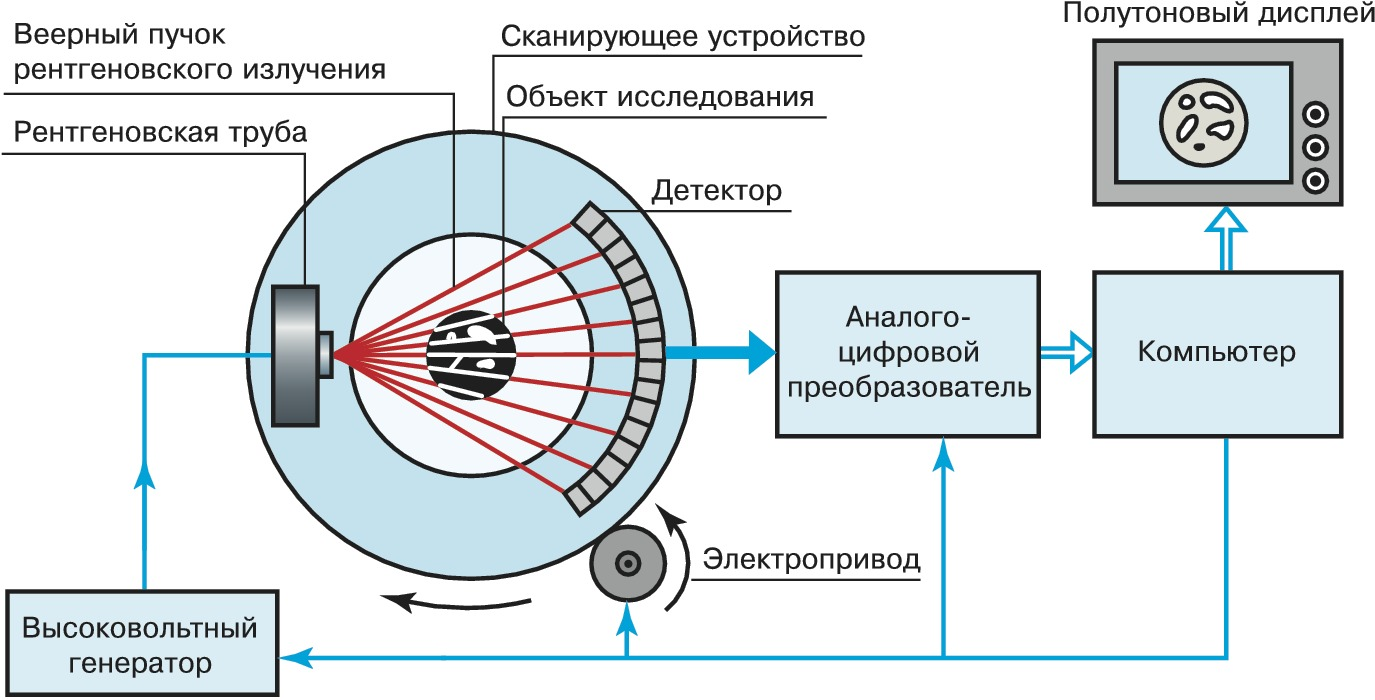
\includegraphics[width=\textwidth]{img/ct.jpeg}
	\caption{Принцип работы компьютерного томографа}
	\label{fig:ct}
\end{figure}

\subsubsection{Магннитно--резонансная томография}

Магнитно--резонансная томография (МРТ) --- это способ получения изображения ядерно--магнитного резонанса, сформулированный в 1973 году профессором университета Иллинойса Полом Лотербуром.

Принцип работы аппарата МРТ основан на воздействии радиосигналов на атомы водорода в челе человека. Будучи помещенными в сильное магнитное поле, атомы резонируют и выдают различные сигналы, на основе анализа которых можно сделать вывод о характере заболевания. Снимки МРТ, которые получаются в результате исследования, позволяют увидеть даже минимальные опухоли и небольшие воспалительные процессы во всех тканях, содержащих воду.

На монитор компьютера выводится трехмерная проекция изучаемого органа, которую можно рассмотреть в любых плоскостях. МР--томограф дает результаты, существенно отличающиеся от получаемых при помощи компьютерной томографии или рентгена. Компьютерная томография ориентирована на изучение физических процессов в мягких тканях, а рентген предназначен для исследования твердых тканей (костей). МРТ позволяет изучать химическое строение тканей и функционирование систем организма в динамике, что позволяет получать полную картину состояния того или иного органа \cite{mrtprinciple}.

На рисунке \ref{fig:mrt} представлен принцип работы магнитно--резонансного томографа.

\begin{figure}[H]
	\centering
	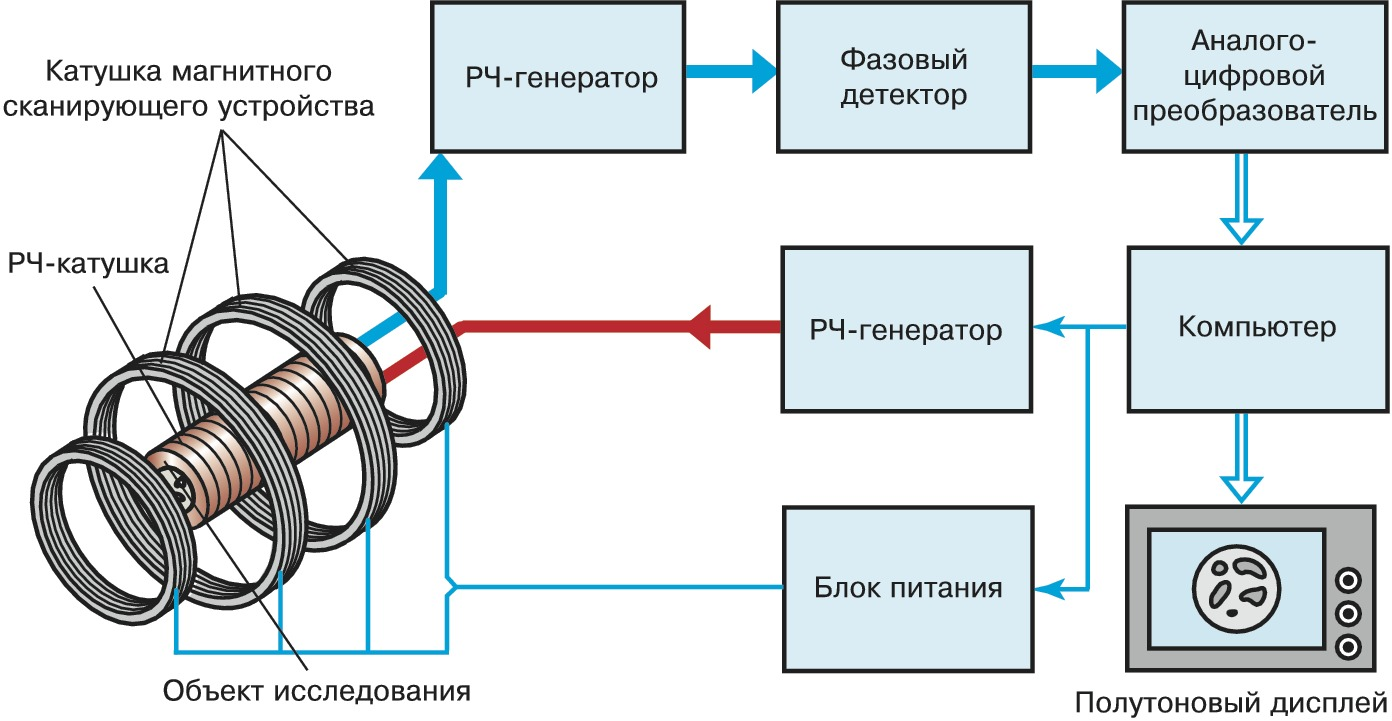
\includegraphics[width=\textwidth]{img/mrt.jpeg}
	\caption{Принцип работы магнитно-резонансного томографа}
	\label{fig:mrt}
\end{figure}

\subsection{Задача распознавания образов}

Задачу распознавания образов можно отнести к задаче классификации \cite{bones}. В контексте работы под образами понимаются кости челюстно--лицевого и зубочелюстнго отделов черепа человека. Классификация является одной из важнейших задач интеллектуального анализа данных. Она решается с помощью аналитических моделей, называемых классификаторами. Востребованность классификации обусловлена сравнительной простотой алгоритмов и методов ее реализации, и высокой интерпретируемостью результатов по сравнению с другими технологиями анализа данных.

В настоящее время разработано большое количество различных видов классификаторов, для построения которых используются как статистические методы (логистическая регрессия, дискриминантный анализ), так и методы машинного обучения (нейронные сети, деревья решений, метод k--ближайших соседей, машины опорных векторов) \cite{classifiers}.

Необходимость использования в анализе данных большого числа разнообразных методов классификации обусловлена тем, что решаемые с ее помощью задачи могут иметь свои особенности, связанные, например, с числом классов (бинарная классификация или классификация с несколькими классами) или с представлением исходных данных --- их объемом, размерностью и качеством, что требует выбора адекватного классификатора. Выбор классификатора, соответствующего особенностям решаемой задачи анализа, является важным фактором получения правильного решения \cite{choice}.

Различные виды классификаторов имеют свои преимущества и недостатки. Так, классификаторы, в которых используются методы статистики имеют хорошую математическую обоснованность, но при этом сложны в использовании и требуют знания вероятностного распределения исходных данных и оценки его параметров, а также имеют фиксированную структуру модели. Такие классификаторы называются параметрическими. Статистические методы оценивают только вероятность принадлежности объекта классу, но не причину этой принадлежности.

Классификаторы, основанные на машинном обучении, не требуют оценки параметров распределения исходных данных, а мера сходства в них формализуется с помощью функции расстояния (обычно, евклидова) \cite{euclidian}. Такие классификаторы называются метрическими. Они проще в реализации и использовании, чем параметрические, а их результаты удобнее для интерпретации. При этом метрические классификаторы представляют собой эвристические модели. Они обеспечивают решение только в ограниченном числе практически значимых случаев, могут дать неточное или не единственное решение.

Компромиссом между параметрическим и метрическими методами является использование для решении задач классификации нейронных сетей. Нейронные сети являются непараметрическими моделями, не требующими предположений о вероятностном распределении данных, но при этом и не используют меры расстояний. Это делает их универсальными классификаторами, позволяя получать результаты даже в случаях, когда параметрические и метрические классификаторы не обеспечиваю приемлемого решения.

\subsection{Задача нахождения объектов на изображении}

Задача нахождения объектов на изображении --- это задача, в рамках которой выполняется определение наличия или отсутствия объекта определённого домена на изображении, нахождение границ этого объекта в системе координат пикселей исходного изображения. 

Данная задача решается при помощи алгоритмов машинного обучения с применением нейронных сетей. В зависимости от алгоритма обучения, объект может характеризоваться координатами ограничивающей рамки, ключевыми точками, контуром объекта.

Задача нахождения объектов на изображении может быть поставлена различным образом и включает в себя класс других задач, помогающих определить, какие объекты находятся на изображении и где они расположены в сетке пикселей исходного изображения.

В контексте работы будут рассмотрены задачи семантической сегментации и сегментации 
экземпляров.

Решением задачи семантической сегментации является признак принадлежности пикселя изображения к определенной категории. Например, если в исходном изображении представлено море, над которым пролетают чайки, то для каждого пикселя необходимо вывести, является ли этот пиксель частью чайки, моря, неба, или какого-то другого типа. Недостаток применения только семантической сегментации относительно задач, связанных с распознаванием объектов --- маркировка пикселей по принадлежности только к типу объекта, что не создаёт различия между объектами как таковыми. Если назвать <<объектом>> связную область пикселей, характеризующих одинаковый тип, то два объекта, перегораживающих друг друга на исходном изображении, будут определены как один объект. В некоторых случаях это приемлемо (как например в задаче данной работы при распознавании зубов в зубочелюстной области). Задача семантической сегментации изображения с дифференцированием объектов называется задачей сегментации экземпляров. Модели, решающие задачу сегментации экземпляров, применяются при необходимости поэкъемплярно отделить распознанные объекты, например, разделить распознанных чаек из представленного примера.

\subsection{Нейронные сети}
\textit{Нейронные сети}, известные также как \textit{искусственные нейронные сети} или \textit{смоделированные нейронные сети}, являются подмножеством алгоритмов машинного обучения и служат основой для алгоритмов глубокого обучения. Понятие <<нейронные сети>> возникло при попытке смоделировать процессы, происходящие в человеческом мозге при передаче сигналов между биологическими нейронами \cite{neuralnet}.

Искусственные нейронные сети состоят из образующих слои узлов: слой входных данных, один или несколько скрытых слоев и слой выходных данных. Каждый узел (искусственный нейрон) связан с другими узлами с определенным весом и пороговым значением. Если вывод какого--либо узла превышает пороговое значение, то этот узел активируется и отправляет данные на следующий уровень сети. В противном случае данные на следующий уровень сети не передаются.

На рисунке \ref{fig:neuralnet} представлена модель работы нейронной сети, где $x_i$ --- входные данные, а $Y_j$ --- выходные данные.

\begin{figure}[H]
	\centering
	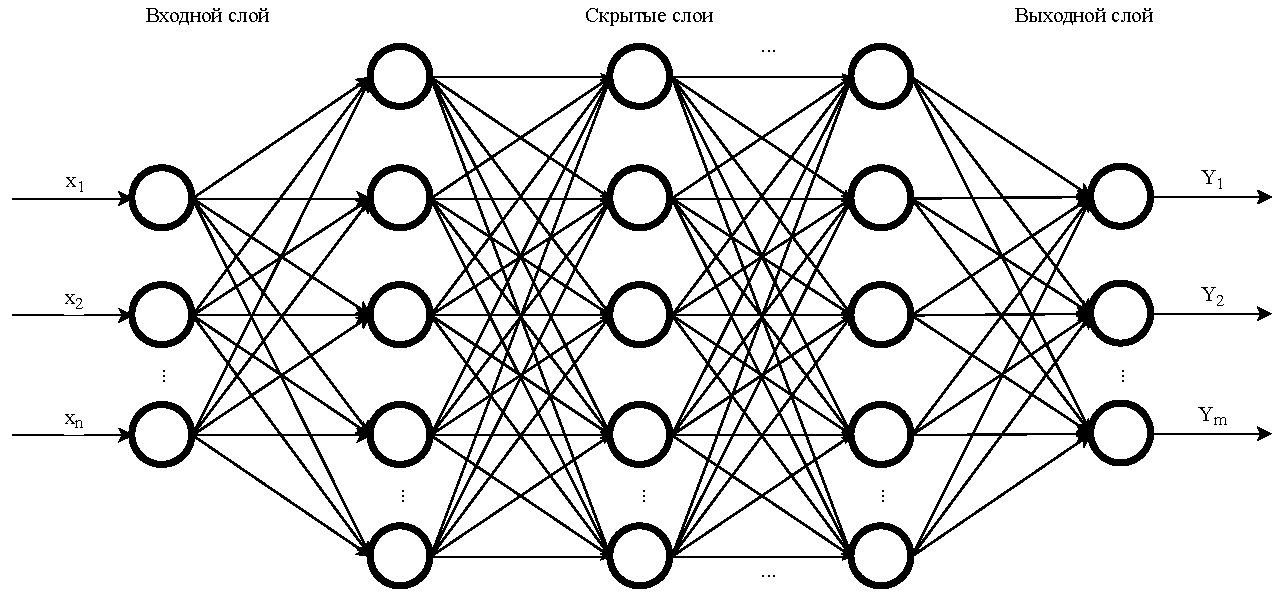
\includegraphics[width=\textwidth]{img/neuralnet.pdf}
	\caption{Модель нейронной сети}
	\label{fig:neuralnet}
\end{figure}

Для обучения и постепенного повышения точности нейронных сетей применяются обучающие данные. При достижении требуемой точности алгоритмы обучения превращаются в мощные инструменты для вычислений и искусственного интеллекта, что позволяет использовать их для классификации и кластеризации данных с высокой скоростью. Задачи из области распознавания речи или изображений можно выполнить за несколько минут, а не за несколько часов, как при распознавании вручную.

\subsubsection{Принцип работы нейронных сетей}

Каждый отдельный узел нейронной сети можно представить в виде модели линейной регрессии \cite{linearreg}, состоящей из входных данных, весовых коэффициентов, смещения (или порогового значения) и выходных данных. Эту модель можно описать следующей формулой:
\begin{equation}
	\label{eq:nn0}
	\hat{y} = \sum_{i=1}^{m}w_ix_i + bias,
\end{equation}
\eqexplSetIntro{где}
\begin{eqexpl}[15mm]
\item{$\hat{y}$} прогнозируемое значение модели;
\item{$m$} количество факторов;
\item{$w$} весовой коэффициент фактора;
\item{$x$} единица входных данных;
\item{$bias$} значение ошибки.
\end{eqexpl}

Выходное значение для узла описывается по формуле:
\begin{equation}
	\label{eq:nn1}
	f(x_i) = \begin{cases}
		1 & \text{если $\hat{y} \ge 0$}\\
		0 & \text{иначе.}\\
		\end{cases}
\end{equation}

После определения слоя входных данных необходимо назначить весовые коэффициенты. Они помогают определить важность фактора: чем выше весовой коэффициент, тем существеннее его вклад в выходные данные по сравнению с другими входными данными. Затем произведения входных данных и соответствующих им весовых коэффициентов суммируются. Наконец, выходные данные передаются через функцию активации \ref{eq:nn1}, которая вычисляет результат. Если полученный результат превышает установленное пороговое значение, узел срабатывает (активируется), передавая данные на следующий слой сети. Выходные данные одного узла становятся входными данными для следующего узла. Такой последовательный процесс передачи данных между слоями характерен для нейронных сетей прямого распространения.

Для более наглядной демонстрации этой концепции рассмотрим реальный пример: допустим, нужно принять решение, стоит ли идти на серфинг (да (1), нет (0)). Решение <<идти>> или <<не идти>> --- прогнозируемый результат $\hat{y}$. Предположим, существует три фактора, которые влияют на принятие решения:

\begin{enumerate}[leftmargin=1.6\parindent]
	\item Хорошие ли сегодня волны? (да (1), нет (0))
	\item Свободна ли зона для плавания? (да (1), нет (0))
	\item Были ли случаи нападения акул в последнее время? (да (1), нет (0))
\end{enumerate}

Предположим, что имеются следующие входные данные:

\begin{itemize}[leftmargin=1.6\parindent]
	\item $x_1 = 1$, так как сегодня хорошие волны для серфинга;
	\item $x_2 = 0$, так как уже собралось много серферов;
	\item $x_3 = 1$, так как в последнее время не было нападений акул.
\end{itemize}

Теперь нужно присвоить весовые коэффициенты для определения важности. Чем выше значение весового коэффициента, тем большим будет влияние конкретной переменной на решение или результат.

\begin{itemize}[leftmargin=1.6\parindent]
	\item $w_1 = 5$, так как большие волны --- редкость;
	\item $w_2 = 2$, так как скопление серферов не является проблемой;
	\item $w_3 = 4$, так как присутствует страх акул.
\end{itemize}

Приняв пороговое значение ($bias$) равным 3 (случайно выбранное значение для примера), можно подставить значения в формулу \ref{eq:nn0} и получить результат.

\begin{equation}
	\label{eq:nn2}
	\hat{y} = (1 * 5) + (0 * 2) + (1 * 4) - 3 = 6.
\end{equation}

С помощью функции активации из формулы \ref{eq:nn1}, можно вычислить выходные данные для этого узла: результат равен 1, так как 6 больше 0. Это означает, что в примере стоит идти на серфинг. Если же изменить весовые коэффициенты или пороговое значение, результат вычисления для данной модели может отличаться. 

Из примера следует, что нейронная сеть способна принимать решения с возрастающей степенью сложности, в зависимости от выходных данных предыдущих решений или слоев. Для иллюстрации математических понятий были использованы персептроны, в то время как в нейронных сетях применяются сигмоидальные нейроны, значения которых могут находиться в диапазоне от 0 до 1. По своему принципу работы нейронные сети схожи с деревьями принятия решений, поэтому в результате передачи данных от одного узла к другому, при $x$ значений от 0 до 1, влияние того или иного изменения отдельной переменной на выходные данные любого узла и, следовательно, выходные данные нейронной сети уменьшается.

В более практических сценариях использования нейронных сетей, например распознавание или классификация изображений, для обучения алгоритма используется контролируемое обучение или маркированные наборы данных. В ходе обучения модели потребуется оценить точность с помощью функции стоимости (среднеквадратическая ошибка). Функция стоимости выражается с помощью формулы:
\begin{equation}
	\label{eq:nn3}
	Cost Function = \frac{1}{2m}\sum_{i=1}^{m}(\hat{y}-y)^2,
\end{equation}
\eqexplSetIntro{где}
\begin{eqexpl}[15mm]
	\item{$i$} индекс выборки;
	\item{$\hat{y}$} прогнозируемое значение;
	\item{$y$} фактическое значение;
	\item{$m$} число выборок.
\end{eqexpl}

Конечная цель --- минимизировать функцию стоимости, чтобы обеспечить корректность для каждого отдельно взятого наблюдения. В процессе корректировки весовых коэффициентов и смещения модель использует функцию стоимости и обучение с подкреплением для достижения точки сходимости или локального минимума. Корректировка весовых коэффициентов происходит с помощью алгоритма градиентного спуска, что позволяет определить стратегию уменьшения количества ошибок (или минимизации функции стоимости). С каждым шагом обучения параметры модели корректируются, пока не будет достигнут минимум. На рисунке \ref{fig:cost} изображен процесс минимизации функции стоимости.

\begin{figure}[H]
	\centering
	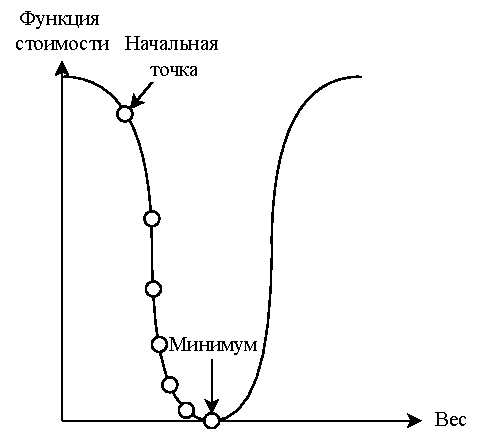
\includegraphics[width=\textwidth]{img/cost.pdf}
	\caption{Минимизация функции стоимости}
	\label{fig:cost}
\end{figure}

Большинство глубоких нейронных сетей относятся к алгоритмам прямого распространения, т. е. данные передаются только в одном направлении --- от входа к выходу. Однако для обучения моделей может также применяться метод обратного распространения ошибки, когда данные передаются в противоположном направлении --- от выхода к входу. Метод обратного распространения ошибки позволяет вычислить и объяснить ошибки, связанные с каждым нейроном, что позволяет скорректировать и адаптировать параметры модели соответствующим образом.

\subsubsection{Метод обратного распространения ошибки}

Метод обратного распространения ошибки (от англ. backpropagation) --- метод вычисления градиента, который используется при обновлении весов в нейронной сети.

Рассмотрим простую нейронную сеть без скрытых слоев (рисунок \ref{fig:simple}), с двумя входными вершинами и одной выходной, в которых каждый нейрон использует линейную функцию активации, которая является взвешенной суммой входных данных.

\begin{figure}[H]
	\centering
	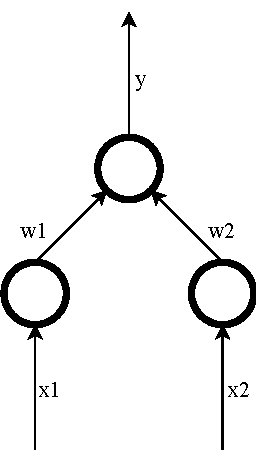
\includegraphics[width=100mm]{img/simple.pdf}
	\caption{Пример нейронной сети}
	\label{fig:simple}
\end{figure}

Изначально веса задаются случайно. Затем, нейрон обучается с помощью тренировочного множества, которое в этом случае состоит из множества троек $(x_1, x_2, \hat{y})$, где $x_1$ и $x_2$ --- это входные данные сети и $\hat{y}$ --- правильный ответ. Начальная сеть, приняв на вход $x_1$ и $x_2$, вычислит ответ $y$, который вероятно отличается от $\hat{y}$. Общепринятый метод вычисления несоответствия между ожидаемым $\hat{y}$ и получившимся $y$ ответом --- квадратичная функция потерь:
\begin{equation}
	\label{eq:nn4}
	E = (\hat{y}-y)^2,
\end{equation}
\eqexplSetIntro{где}
\begin{eqexpl}[15mm]
	\item{$E$} ошибка.
\end{eqexpl}

В качестве примера, обучим сеть на объекте $(1, 1, 0)$, таким образом, значения $x_1$ и $x_2$ равны 1, а $\hat{y}$ равно 0. Построим график зависимости ошибки $E$ от действительного ответа $y$, его результатом будет парабола (рисунок \ref{fig:error}).

\begin{figure}[H]
	\centering
	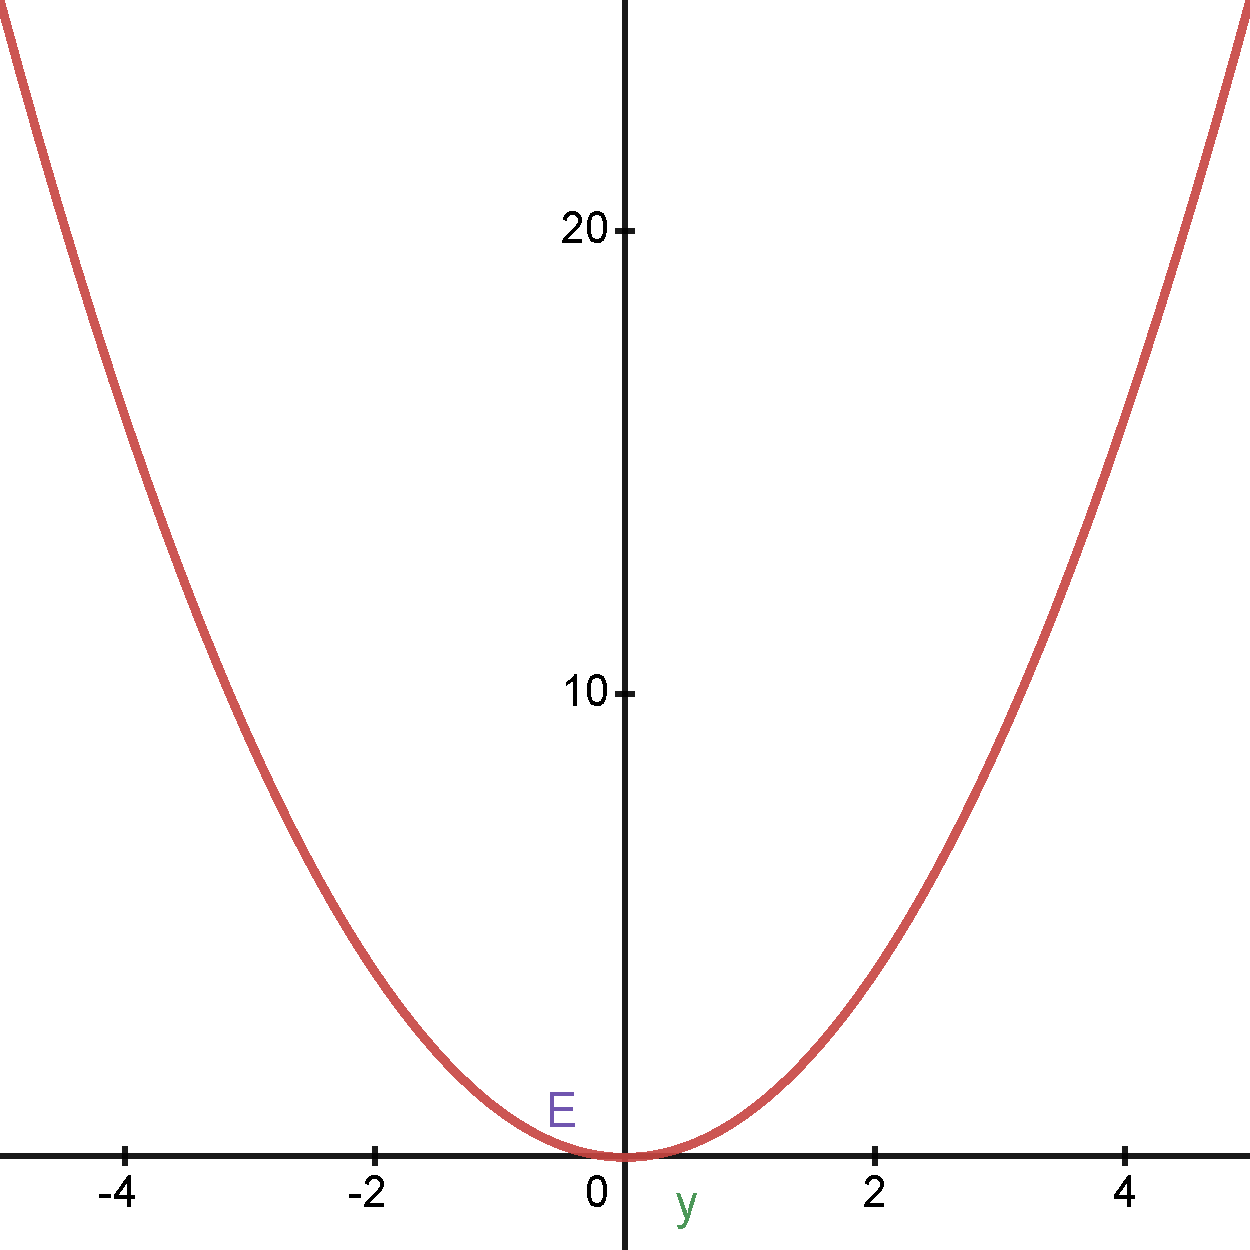
\includegraphics[width=\textwidth]{img/error.pdf}
	\caption{Зависимость ошибки от действительного ответа}
	\label{fig:error}
\end{figure}

Минимум параболы соответствует ответу $y$, минимизирующему $E$. Если тренировочный объект один, минимум касается горизонтальной оси, следовательно ошибка будет нулевая и сеть может выдать ответ $y$, равный ожидаемому ответу $\hat{y}$. Следовательно, задача преобразования входных значений в выходные может быть сведена к задаче оптимизации, заключающейся в поиске функции, которая даст минимальную ошибку.

В таком случае, выходное значение нейрона --- взвешенная сумма всех его входных значений:
\begin{equation}
	\label{eq:nn5}
	\hat{y} = x_1w_1 + x_2w_2,
\end{equation}
\eqexplSetIntro{где}
\begin{eqexpl}[15mm]
	\item{$w_1, w_2$} веса на ребрах, соединяющих входные вершины с выходной.
\end{eqexpl}

Следовательно, ошибка зависит от весов ребер, входящих в нейрон. Именно это нужно менять в процессе обучения. Распространенный алгоритм для поиска набора весов, минимизирующего ошибку --- градиентный спуск, описанный ранее. Метод обратного распространения ошибки используется для вычисления самого крутого направления для спуска.

\subsubsection{Виды нейронных сетей}

Нейронные сети можно разделить на несколько видов, в зависимости от целевого назначения. 

\textit{Персептрон} --- первая нейронная сеть, созданная Фрэнком Розентблаттом в 1958 году. Она содержит один нейрон и представляет собой простейшую форму нейронной сети. На рисунке \ref{fig:perceptron} изображен пример такой нейронной сети.

\begin{figure}[H]
	\centering
	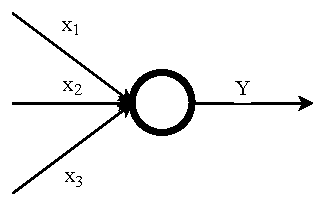
\includegraphics[width=\textwidth]{img/perceptron.pdf}
	\caption{Персептрон}
	\label{fig:perceptron}
\end{figure}

\textit{Нейронные сети прямого распространения (многослойные персептроны (MLP)} --- нейронные сети, состоящие из слоев входных данных, одного или нескольких скрытых слоев и выходных данных. Данные, поступающие в эти модели, используются для обучения. Эти сети лежат в основе алгоритмов компьютерного зрения, обработки данных на естественном языке и других нейронных сетей.

\textit{Рекуррентные нейронные сети (RNN)} имеют в своем составе обратные связи. Такие алгоритмы обучения используются в основном для временных рядов данных с целью прогнозирования будущих событий, например стоимости акций на фондовых биржах или объема продаж.

\subsubsection{Сравнение нейронных сетей и глубокого обучения}

Часто термины <<глубокое обучение>> и <<нейронные сети>> могут использоваться как синонимы, что не совсем верно. Стоит отметить, что понятие <<глубина>> в <<глубоком обучении>> характеризует лишь количество слоев нейронной сети. Нейронную сеть, в составе которой более трех слоев (включая слой входных данных и слой выходных данных), можно отнести к алгоритмам глубокого обучения. Нейронная сеть с двумя--тремя уровнями считается простой нейронной сетью.

\subsubsection{Особенности применения нейронных сетей в качестве классификаторов}

Задача классификации для нейронных сетей не является основной. Основной задачей для нейронных сетей является численное предсказание (как было показано на примере с серфингом).

Используя специальные способы представления данных, можно адаптировать нейронные сети для работы с категориальными данными, т.е. получать на вход и формировать на выходе категориальные значения. Для этого категориальные признаки соответствующим образом кодируются с помощью числовых значений.

Нейронные сети имеют ряд преимуществ при использовании в качестве классификаторов. Например:
\begin{itemize}[leftmargin=1.6\parindent]
	\item нейронные сети являются самообучаемыми моделями, работа которых практически не трубет вмешательства пользователя;
	\item нейронные сети являются универсальными аппроксиматорами, позволяющими аппроксимировать любую непрерывную функцию с приемлемой точностью;
	\item нейронные сети являются нелинейными моделями, что позволяет эффективно решать задачи классификации даже при отсутствии линейной разделимости классов. На рисунке \ref{fig:separation} приведен пример линейной разделимости и неразделимости классов.
\end{itemize}

\begin{figure}[H]
	\centering
	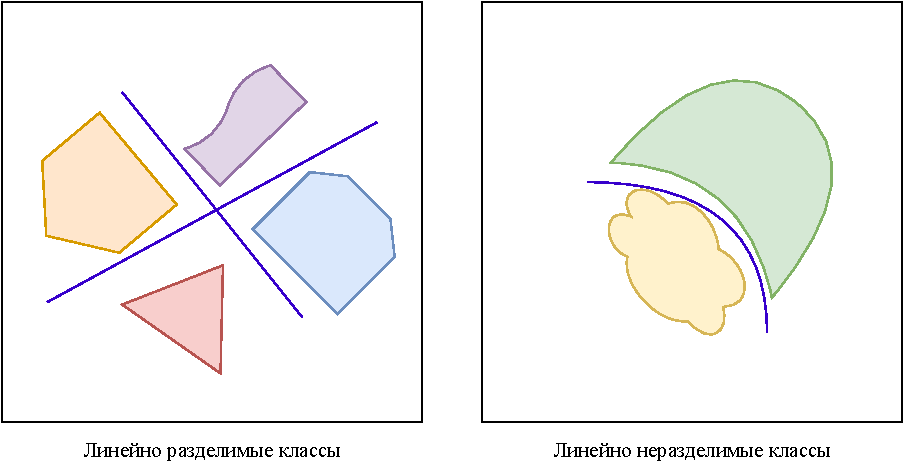
\includegraphics[width=\textwidth]{img/separation.pdf}
	\caption{Линейная разделимость классов}
	\label{fig:separation}
\end{figure}

Следует отметить, что каких--либо специальных нейросетевых архитектур для классификации не существует. Наиболее часто используемой для классификации архитектурой нейронных сетей являются сети прямого распространения, на входные нейроны которых подаются значения признаков классифицируемого объекта, а на выходе формируется метка или числовой код класса.

Последующие слои, таким образом, разделяют объекты на классы в пространстве признаков более высокой размерности, чем исходное. Например, если размерность вектора признаков исходных данных равна 4, и скрытый слой содержит 6 нейронов, то выходной слой производит разбиение объектов на классы в 6--мерном пространстве.

Это позволяет сделать процесс более эффективным: правильно подобрав конфигурацию и параметры нейронной сети, можно получить хорошие результаты классификации даже в тех случаях, когда классификаторы других типов, работающие только в размерности обучающих данных, не обеспечивают приемлемых результатов. Недостатком является то, что конфигурация сети, наилучшим образом аппроксимирующая функцию разделения классов в пространстве признаков, заранее неизвестна. Поэтому приходится подбирать её экспериментально, либо использовать опыт аналогичных решений.

Если распределение классов таково, что для их разделения требуется сложная функция, размерность нейронной сети может оказаться неприемлемо большой. В этом случае проблему можно решить с помощью специальной предобработки исходных данных.

\subsubsection{Машина опорных векторов}

SVM (от англ. Support vector machine) --- метод машинного обучения, применяемый в задачах классификации, основанный на построении гиперплоскости и ее анализе \cite{svm}.

Главная цель SVM как классификатора --- найти уравнение разделяющей гиперплоскости $w_1x_1+w_2x_2+…+w_nx_n+w_0=0$ в пространстве $R^n$, которая бы разделила два класса неким оптимальным образом. Общий вид преобразования $F$ объекта $x$ в метку класса $Y$ представлен в формуле \ref{eq:nn6}: 
\begin{equation}
	\label{eq:nn6}
	F(x) = sign(w^Tx-b),
\end{equation}

При рассмотрении обозначим $w = (w_1, w_2, …, w_n), b=-w_0$. После настройки весов алгоритма $w$ и $b$, все объекты, попадающие по одну сторону от построенной гиперплоскости, будут предсказываться как первый класс, а объекты, попадающие по другую сторону --- второй класс.

Внутри функции $sign()$ стоит линейная комбинация признаков объекта с весами алгоритма, именно поэтому SVM относится к линейным алгоритмам. Разделяющую гиперплоскость можно построить разными способами, но в SVM веса $w$ и $b$ настраиваются таким образом, чтобы объекты классов лежали как можно дальше от разделяющей гиперплоскости. Другими словами, алгоритм максимизирует зазор (англ. margin) между гиперплоскостью и объектами классов, которые расположены ближе всего к ней. Такие объекты и называют опорными векторами.

На рисунке \ref{fig:svm1} представлен принцип работы машины опорных векторов.

\begin{figure}[H]
	\centering
	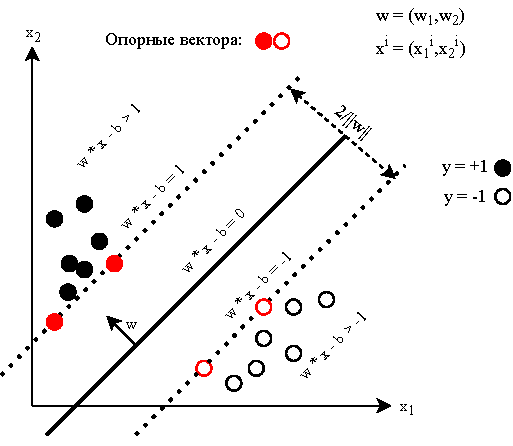
\includegraphics[width=\textwidth]{img/svm1.pdf}
	\caption{Визуализация работы SVM}
	\label{fig:svm1}
\end{figure}

Чтобы разделяющая гиперплоскость как можно дальше отстояла от точек выборки, ширина полосы должна быть максимальной. Вектор $w$ --- вектор нормали к разделяющей гиперплоскости. Здесь и далее скалярное произведение двух векторов будет обозначаться как $\langle a,b\rangle$ или $a^Tb$. Проекция вектора $w$, концами которого являются опорные вектора разных классов, будет показывать ширину разделяющий полосы.

На рисунке \ref{fig:svm2} представлен вывод правил настройки весов.

\begin{figure}[H]
	\centering
	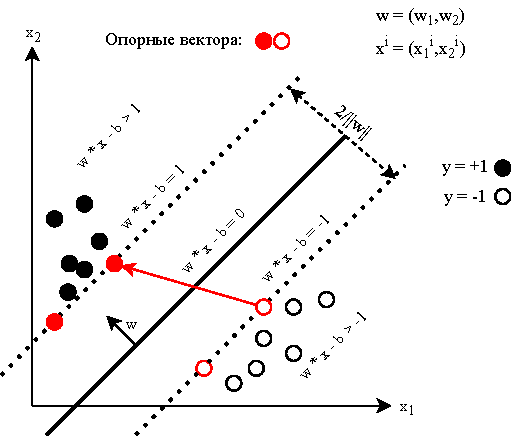
\includegraphics[width=\textwidth]{img/svm2.pdf}
	\caption{Вывод правил настройки весов}
	\label{fig:svm2}
\end{figure}

В формулах \ref{eq:nn7} --- \ref{eq:nn10} представлен вывод правил настройки весов.

\begin{equation}
	\label{eq:nn7}
	\langle(x_+-x_-),\frac{w}{\Arrowvert w\Arrowvert}\rangle = \frac{\langle x_+,w\rangle - \langle x_-,w\rangle}{\Arrowvert w\Arrowvert} = \frac{(b+1)-(b-1)}{\Arrowvert w\Arrowvert} = \frac{2}{\Arrowvert w\Arrowvert},
\end{equation}

\begin{equation}
	\label{eq:nn8}
	\frac{2}{\Arrowvert w\Arrowvert} \rightarrow max,
\end{equation}

\begin{equation}
	\label{eq:nn9}
	\Arrowvert w\Arrowvert \rightarrow min,
\end{equation}

\begin{equation}
	\label{eq:nn10}
	\frac{w^Tw}{2} \rightarrow min.
\end{equation}

Отступом (англ. margin) объекта $x$ от границы классов называется величина $M=y(w^Tx-b)$. Алгоритм допускает ошибку на объекте тогда и только тогда, когда отступ $M$ отрицателен (когда $y$ и $w^Tx-b$ разных знаков). Если $M ∈ (0, 1)$, то объект попадает внутрь разделяющей полосы. Если $M > 1$, то объект $x$ классифицируется правильно, и находится на некотором удалении от разделяющей полосы. Алгоритм будет правильно классифицировать объекты, если выполняется условие, представленное в формуле \ref{eq:nn11}.

\begin{equation}
	\label{eq:nn11}
	y(w^Tx-b) \geq 1
\end{equation}

\subsection{Методы и технологии распознавания образов}

Для решения задачи распознавания образов с помощью нейронных сетей применяются такие способы, как:
\begin{itemize}[leftmargin=1.6\parindent]
	\item R--CNN (от англ. Region--based Convolutional Network);
	\item Fast R--CNN;
	\item Faster R--CNN. 
\end{itemize}

\subsubsection{R--CNN}

R--CNN имеет следующую схему работы:
\begin{enumerate}[leftmargin=1.6\parindent]
	\item При помощи \textit{selective search} (с англ. избирательный поиск)  \cite{selsearch} на изображении выделяются регионы, которые предположительно содержат объект (кости лица на КТ или МРТ снимке).
	\item Регион--претендент при помощи аффинного преобразования отображается в квадрат 227$\times$227.
	\item Полученный прямоугольник подается на вход сети \cite{imagenet}, которая имеет структуру, представленную на рисунке \ref{fig:rcnn}.
	 \begin{figure}[H]
	 	\centering
	 	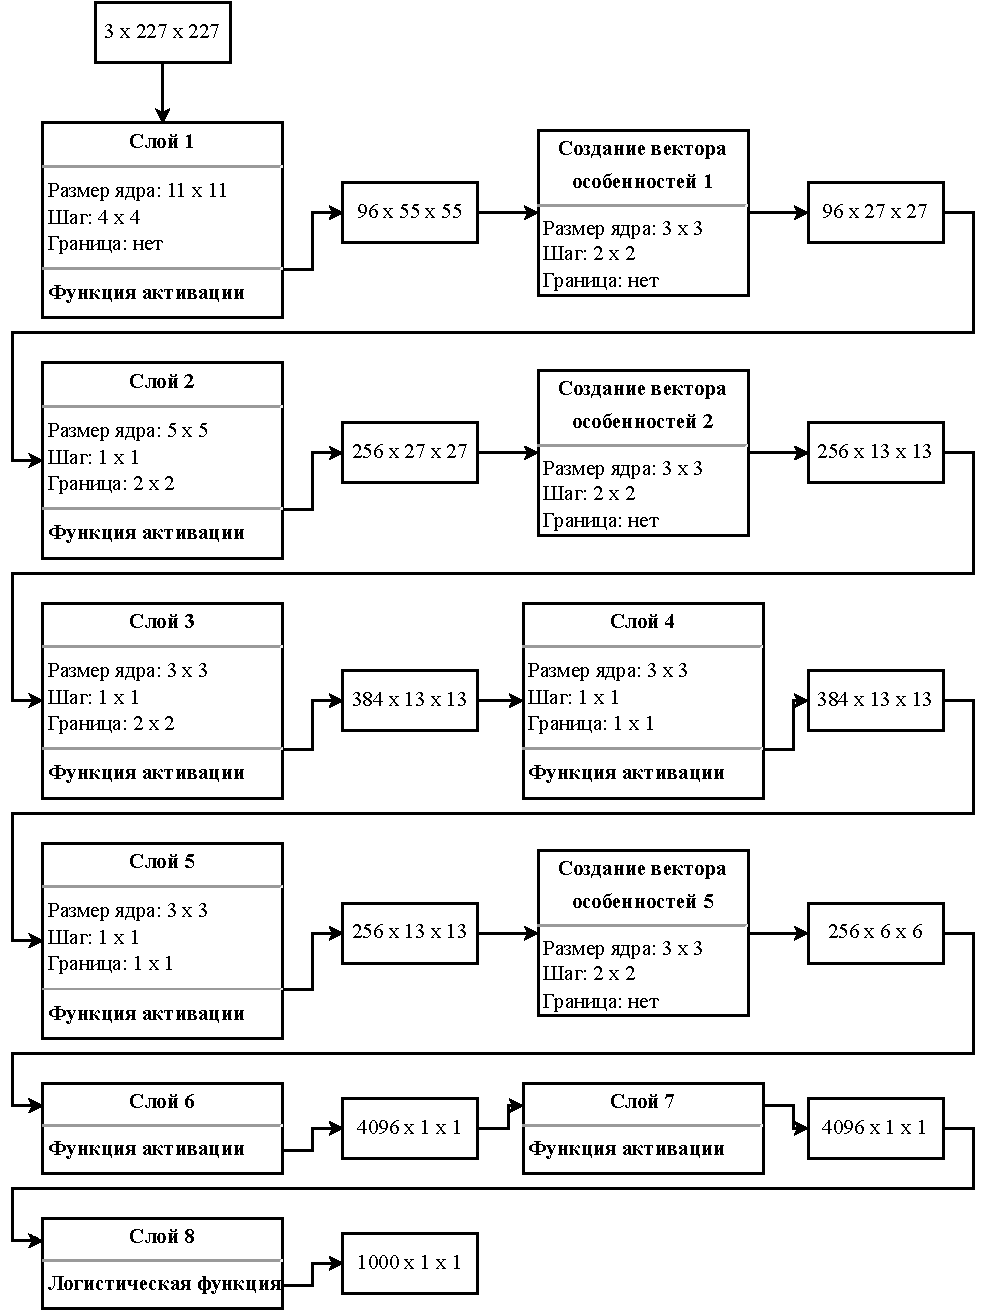
\includegraphics[width=\textwidth]{img/rcnn.pdf}
	 	\caption{Принцип работы R--CNN}
	 	\label{fig:rcnn}
	 \end{figure}
 	\item С седьмого слоя сети снимается вектор размерности 4096. Этот вектор используется в машине опорных векторов, натренированной для каждого класса, для классификации.
 	\item Вектор подается в линейный регрессор (логистическая функция), соответствующий классу объекта для восстановления позиции объекта.
\end{enumerate}

\subsubsection{Fast R--CNN}

R--CNN имеет несколько недостатков, в основном связанных с высокими временными затратами:
\begin{enumerate}[leftmargin=1.6\parindent]
	\item Требуется натренировать сверточную нейронную сеть (в два этапа: тренировка без точной разметки и оптимизация для 20 классов).
	\item Требуется натренировать набор машин опорных векторов по одной для каждого класса. При этом на вход машина опорных векторов принимает вектора особенностей, полученных от натренированной сверточной сети. Эти вектора нужно изначально вычислить на наборе данных, используемых для тренировки.
	\item Требуется натренировать линейные регрессоры (по одному для каждого класса) для восстановления позиций объекта.
	\item Процесс детектирования и классификации требует существенного времени (до 49 секунд на одно изображение) \cite{fastrcnn}.
\end{enumerate}

Существенные временные затраты на этапе детектирования сильно снижают практическую пользу R--CNN. Причина, из--за которой детектирование работает так медленно, заключается в том, что при помощи избирательного поиска генерируется примерно 2000 претендентов на изображении, и каждый претендент должен быть пропущен через сверточную сеть, чтобы вычислить для него вектор особенностей. Процесс этот достаточно затратный, особенно для сетей с большим числом сверточных слоев. В Fast R--CNN предлагают подавать на вход сети полное изображение, но при этом последний слой заменить на слой типа \textit{RoI pooling} (Region of Interest Pooling) \cite{fastrcnn}.

\textit{RoI pooling} слой принимает на вход карту особенностей, полученную от последнего сверточного слоя нейронной сети, и RoI претендента (в координатах изображения). RoI преобразуется из координат изображения в координаты на карте особенностей и на полученный прямоугольник накладывается сетка $W \times H$ с наперед задаными размерами (например, $W = H = 7$) \cite{fastrcnn}. RoI pooling слой преобразует вектор особенностей произвольного прямоугольника из исходного изображения в вектор особенностей фиксированной размерности.

После RoI pooling слоя данные через два полносвязных слоя подаются параллельно на слой для оценки принадлежности претендента одному из классов объектов и слой, реализующий регрессию для уточнения границы объекта.

Итоговый принцип работы Fast R--CNN представлен на рисунке \ref{fig:fastrcnn}.

\begin{figure}[H]
	\centering
	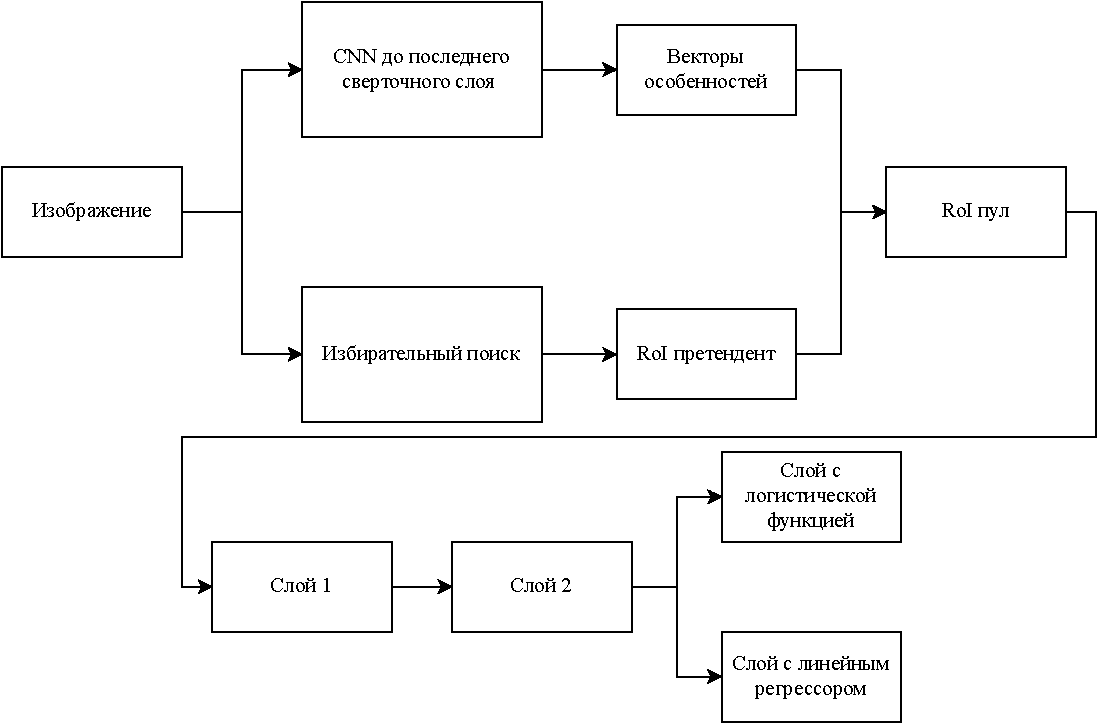
\includegraphics[width=\textwidth]{img/fastrcnn.pdf}
	\caption{Принцип работы Fast R--CNN}
	\label{fig:fastrcnn}
\end{figure}

В отличии от R--CNN, где карта особенностей генерировалась для каждого претендента на изображении, в Fast R--CNN генерируется карта особенностей для всего изображения, а затем при помощи специального слоя из нее вычленяются карты для каждого из претендентов, что позволяет существенно сократить время вывода.

\subsubsection{Faster R--CNN}

В качестве улучшения Fast R--CNN предлагается замена процедуры генерации претендентов избирательным поиском на нейронную сеть, которая использует имеющуюся карту особенностей (для примера, VGG16) \cite{fasterrcnn}. Для изображения размера $W_1 \times H_1$ на выходе последнего сверточного слоя сеть VGG16 выдает карту особенностей с размерами $W_1/16 \times H_1/16$, вектор особенностей для каждой точки будет иметь размерность 512. При этом вектор особенностей в точке ($x_f, y_f$) вносят вклад точки изображения, лежащие внутри квадрата с центром в ($16x_f, 16y_f$) и размера 196 $\times$ 196.

Для каждой точки карты особенностей ($x_f, y_f$) проверяется $k$ претендетов разных размеров на изображении в регионах с центром в ($16x_f, 16y_f$). Рассматривают 9 претендентов, варьируя три масштаба и три отношения сторон ($1\div1, 1\div2, 2\div1$). Для решения задачи используется \textit{Region Proposal Network (RPN)} (от англ. сеть для предложения регионов) \cite{rpn}.

Итоговый принцип работы Faster R--CNN представлен на рисунке \ref{fig:fasterrcnn}.

\begin{figure}[H]
	\centering
	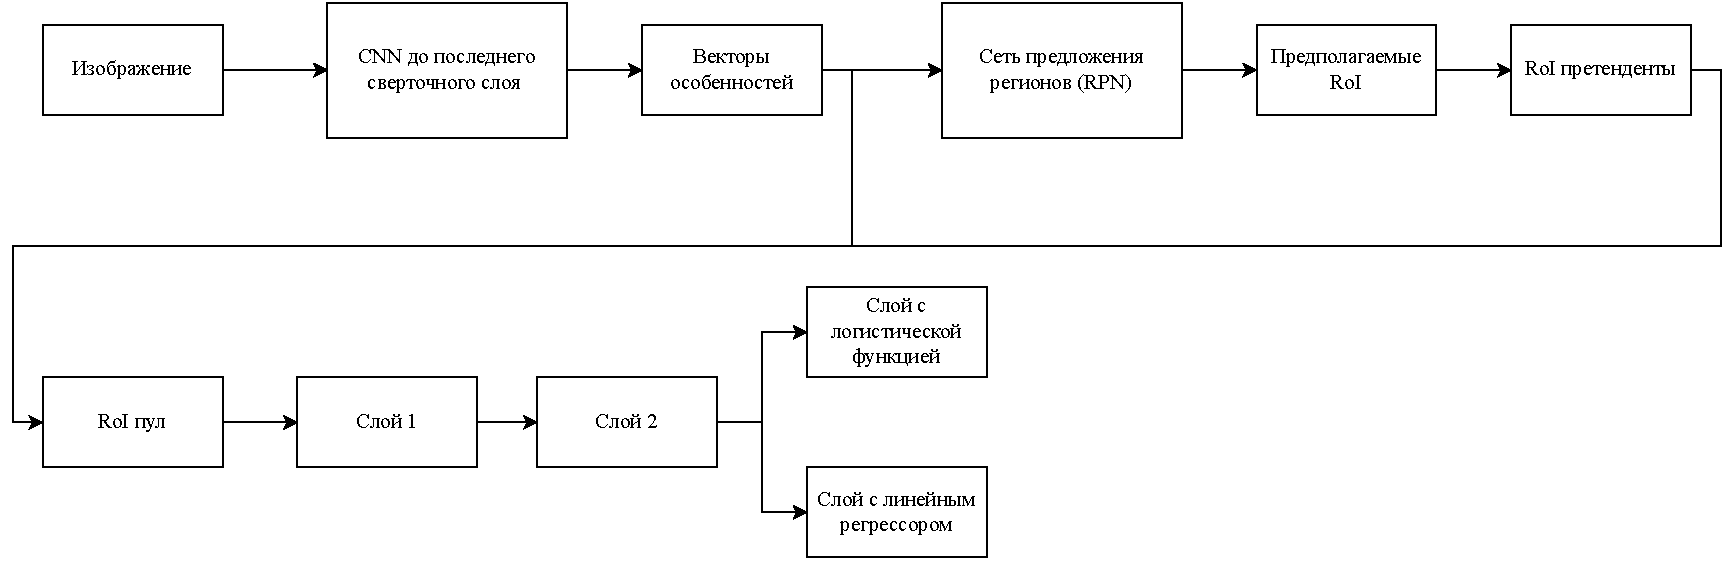
\includegraphics[width=\textwidth]{img/fasterrcnn.pdf}
	\caption{Принцип работы Faster R--CNN}
	\label{fig:fasterrcnn}
\end{figure}

Замена генерации претендентов избирательным поиском на нейронную сеть позволяет повысить быстродействие распознавания образов на изображений до десяти раз \cite{fasterrcnn}.

\subsubsection{Сравнение рассмотренных методов}

Сравнительная характеристика рассмотренных методов представлена в таблице \ref{tab:reccomp}.

% Please add the following required packages to your document preamble:
% \usepackage{graphicx}
\begin{table}[H]
	\centering
	\caption{Сравнение методов распознавания образов}
	\label{tab:reccomp}
	\resizebox{\textwidth}{!}{%
		\begin{tabular}{|l|l|l|l|}
			\hline
			\textbf{Критерий}                     & \textbf{R–CNN} & \textbf{Fast R--CNN} & \textbf{Faster R--CNN} \\ \hline
			Время распознавания, сек*             & $\sim$49       & 2.32                & 0.2                   \\ \hline
			Время вычисления                      & Высокое        & Высокое             & Низкое                \\ \hline
			mAP** на датасете Pascal VOC 2007, \% & 58.5           & 66.9                & 69.9                  \\ \hline
			mAP** на датасете Pascal VOC 2012, \% & 53.3           & 65.7                & 67.0                  \\ \hline
		\end{tabular}%
	}
\end{table}
* --- меньше --- лучше.

** --- mAP (от англ. mean average precision) --- метрика измерения точности обнаруживаемых объектов. Больше --- лучше.

\subsection{Методы и технологии выделения объектов на изображении}

Для решения задачи распознавания образов с помощью нейронных сетей применяются такие способы, как:
\begin{itemize}[leftmargin=1.6\parindent]
	\item Mask R--CNN;
	\item UNet. 
\end{itemize}

\subsubsection{Mask R--CNN}

Mask R--CNN развивает архитектуру Faster R--CNN путём добавления ещё одной ветки, которая предсказывает положение маски, покрывающей найденный объект, и, таким образом решает уже задачу сегментации экземпляров. Маска представляет собой просто прямоугольную матрицу, в которой 1 на некоторой позиции означает принадлежность соответствующего пикселя объекту заданного класса, 0 --- что пиксель объекту не принадлежит.

Архитектура Mask R--CNN условно разделяется на CNN--сеть вычисления признаков изображения, называемую backbone, и head --- объединение частей, отвечающих за предсказание охватывающей рамки, классификацию объекта и определение его маски. Функция потери для них общая и включает три компонента:

\begin{equation}
	\label{eq:nn11}
	L = L_{cls} + L_{box} + L_{mask},
\end{equation}
\eqexplSetIntro{где}
\begin{eqexpl}[15mm]
	\item{$L_{cls}$} функция потери для этапа классификации;
	\item{$L_{box}$} функция потери для этапа выделения охватывающей рамки;
	\item{$L_{mask}$} функция потери для этапа определения маски;
\end{eqexpl}

Маски предсказываются отдельно для каждого класса, без предварительного знания, что изображено в регионе, и потом выбирается маска класса, победившего в независимом классификаторе. Утверждается, что такой подход более эффективен, чем опирающийся на априорное знание класса.

Одна из основных модификаций, возникших из--за необходимости предсказывать маску --- изменение процедуры RoIPool (вычисляющей матрицу признаков для региона--кандидата) на процедуру RoIAlign. Дело в том, что карта признаков, полученная из CNN, имеет меньший размер, чем исходное изображение, и регион, охватывающий на изображении целочисленное количество пикселей, не получается отобразить в пропорциональный регион карты с целочисленным количеством признаков (рисунок \ref{fig:maskrcnn}). 

\begin{figure}[H]
	\centering
	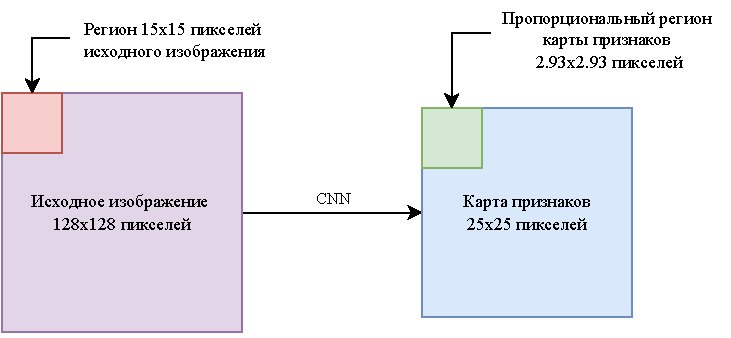
\includegraphics[width=\textwidth]{img/maskrcnn.pdf}
	\caption{Проблема отображения региона изображения в регион карты}
	\label{fig:maskrcnn}
\end{figure}

В RoIPool проблема решалась округлением дробных значений до целых. Такой подход нормально работает при выделении охватывающей рамки, но вычисленная на основе таких данных маска получается неточной.

В RoIAlign не используется округление, все числа остаются действительными, а для вычисления значений признаков используется билинейная интерполяция по четырём ближайшим целочисленным точкам.

\subsubsection{UNet}

UNet считается одной из стандартных архитектур CNN для задач сегментации изображений, когда нужно не только определить класс изображения целиком, но и сегментировать его области по классу (сегментация экземпляров). Архитектура сети состоит из стягивающего пути для захвата контекста и симметричного расширяющегося пути, который позволяет осуществить точную локализацию \cite{unet}.

На рисунке \ref{fig:unet} представлена архитектура UNet.

\begin{figure}[H]
	\centering
	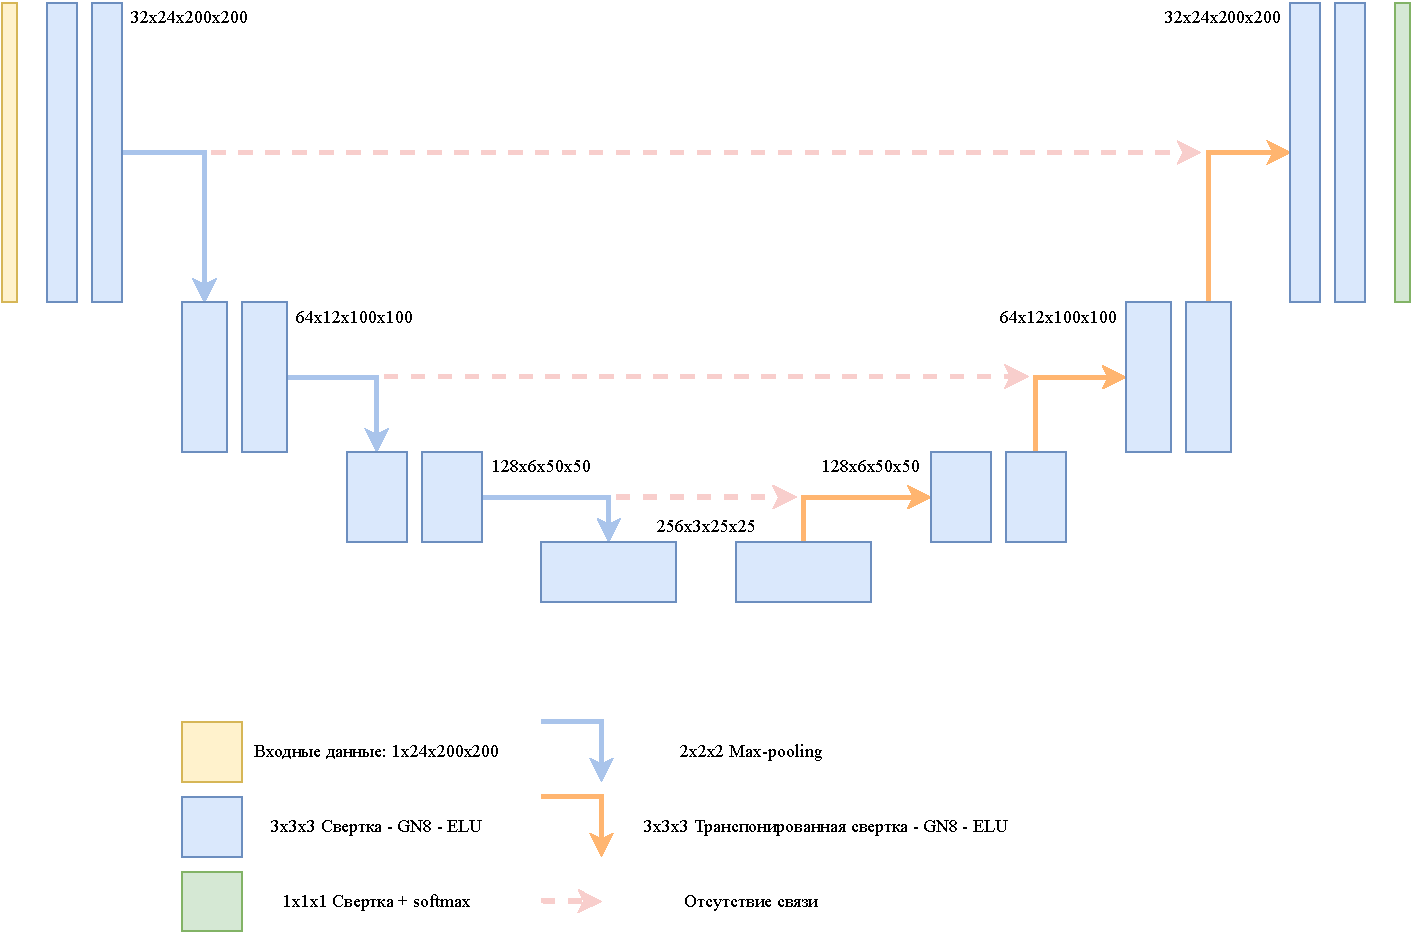
\includegraphics[width=\textwidth]{img/unet.pdf}
	\caption{Принцип работы UNet}
	\label{fig:unet}
\end{figure}

Сеть обучается сквозным способом на небольшом количестве изображений Сегментация изображения размером $512 \times 512$ пикселей занимает менее секунды на современном графическом процессоре (например, Nvidia GeForce RTX 3050).

UNet состоит из сужающегося пути (слева) и расширяющегося пути (справа). Сужающийся путь состоит из повторного применения двух сверток $3 \times 3$, за которыми следует функция активации ReLU (от англ. Rectified Linear Unit) и операция максимального объединения для понижения разрешения.

На каждом этапе понижающей дискретизации каналы свойств удваиваются. Каждый шаг в расширяющемся пути состоит из операции повышающей дискретизации карты свойств, за которой следуют:
\begin{itemize}
	\item свертка $2 \times 2$, которая уменьшает количество каналов свойств;
	\item объединение с обрезанной картой свойств из сужающегося пути;
	\item две $3 \times 3$ свертки, за которыми следует функция активации ReLU.
\end{itemize}

Обрезка необходима из-за потери граничных пикселей при каждой свертке.

На последнем слое используется свертка $1 \times 1$ для сопоставления каждого 64--компонентного вектора свойств с желаемым количеством классов. Всего сеть содержит 23 сверточных слоя.

\subsubsection{Сравнение рассмотренных методов}

Согласно исследованиям \cite{segcomp} при сравнении Mask R--CNN и UNet Mask R--CNN показала большую точность в сравнении с UNet ($0.76 \pm 0.03$ против $0.43 \pm 0.12$). Несмотря на это, UNet применяется в большей части биомедицинских задач. Это означает, что существует большее число моделей и возможных подходов при тренировке модели.

\subsubsection*{Вывод}

Были рассмотрены медицинские методы томографии.

Была рассмотрены задача распознавания образов (классификации) и выделения объектов на изображении (сегментации), виды классификаторов и их применимость при распознавании образов.

Было дано определение понятия нейронной сети, рассмотрены виды нейронных сетей и принцип их работы.

Были рассмотрены особенности применения нейронных сетей в качестве классификаторов.

Были рассмотрены и проанализированы технологии (R--CNN, Fast R--CNN и Faster R--CNN) для распознавания образов при помощи нейронных сетей и для выделения объектов на изображений (Mask R--CNN, UNet), приведены преимущества и недостатки рассмотренных технологий.

В качестве базовых технологии для разрабатываемого метода выбраны модель нейронной сети UNet, так как она широко используется в биомедицинских задачах и дает приемлемый результат по затраченному времени как при обучении, так и при сегментации изображения. Для посткласификации распознанных костей выбрана технология машины опорных векторов. При полученной сегментации можно составить векторы свойств сегментированных изображений и применить метод опорных векторов для дальнейшей классификации.